
%(BEGIN_QUESTION)
% Copyright 2009, Tony R. Kuphaldt, released under the Creative Commons Attribution License (v 1.0)
% This means you may do almost anything with this work of mine, so long as you give me proper credit

Calculate the percentage of incident power reflected back to the transmitter, and the percentage of incident power transmitted (forward) through the liquid in this radar level measurement application:

$$\includegraphics[width=15.5cm]{i04216x01.eps}$$

Also, calculate the ullage for this vessel in both units of meters and units of feet/inches, given a reflected pulse (``echo'') time of 11.176 nanoseconds.  Note: the propagation velocity of radio waves in air is approximately $3 \times 10^8$ meters per second, the same as the speed of light in a vacuum.

\vskip 20pt \vbox{\hrule \hbox{\strut \vrule{} {\bf Suggestions for Socratic discussion} \vrule} \hrule}

\begin{itemize}
\item{} An effective problem-solving technique to apply to the calculation of ullage is to {\it simplify the problem} and solve that simplified problem.  In this case, an easy way to ``simplify the problem'' is to change the numerical values for echo time and speed of light until the solution for ullage becomes obvious even without using a calculator.  Then the formula we must use to calculate {\it any} time/speed/ullage echo problem will be apparent.  Apply the ``simplify the problem'' technique to this ullage calculation.
\item{} Would you say this is an example of good signal reflection, or poor signal reflection?  In general terms, what condition(s) make for strong reflected signals for a radar-based level instrument?
\end{itemize}

\underbar{file i04216}
%(END_QUESTION)





%(BEGIN_ANSWER)

\noindent
{\bf Partial answer:}

\vskip 10pt

$P_{reflected}$ = 63.45\%

\vskip 10pt

Ullage = 1.676 meters

%(END_ANSWER)





%(BEGIN_NOTES)

The relationship between velocity ($v$), time ($t$), and distance ($x$) for any traveling wave is as follows:

$$x = vt$$

Thus, for a wave traveling at $2.9979 \times 10^8$ m/s over a time of 11.176 ns, the total distance traveled will be:

$$x = (2.9979 \times 10^8 \hbox{ m/s})(11.176 \hbox{ ns})$$

$$x = 3.3505 \hbox{ m}$$

This, of course is the {\it total} travel distance for the wave, from the transmitter, to the air/water interface, and back to the transmitter.  The ullage will be one-half of this round-trip distance:

$$\hbox{Ullage} = 1.6752 \hbox{ m}$$

Converting this ullage into English units, we get 5.496 feet, or {\bf 5 feet 5.95 inches}.

\vskip 10pt

The amount of signal reflection off the air/water interface may be calculated using this formula:

$$R = {\left({\sqrt{\epsilon_{r}} - 1}\right)^2 \over \left(\sqrt{\epsilon_{r}} + 1 \right)^2}$$

Plugging in our values of $\epsilon$ for the water, we get:

$$R = {\left({\sqrt{78} - 1}\right)^2 \over \left(\sqrt{78} + 1 \right)^2}$$

$$R = 0.6345$$

Thus, the air/water interface will reflect 63.45\% of the incident signal, allowing 36.45\% of that signal to pass through into the water.

\vskip 10pt

The 87 $^{o}$F air temperature is extraneous information, included for the purpose of challenging students to identify whether or not information is relevant to solving a particular problem.




\vfil \eject

\noindent
{\bf Summary Quiz:}

Suppose a radar wave takes 56 nanoseconds to travel to an object, reflect back, and return to its source while traveling through air.  How far away is the object from the radar transceiver, in meters?

\begin{itemize}
\item{} 187 meters
\vskip 5pt 
\item{} 28 meters
\vskip 5pt 
\item{} 93.3 meters
\vskip 5pt 
\item{} 56 meters
\vskip 5pt 
\item{} 8.4 meters
\vskip 5pt 
\item{} 16.8 meters
\end{itemize}

%INDEX% Measurement, level: radar

%(END_NOTES)


